\documentclass{article}\usepackage[]{graphicx}\usepackage[]{xcolor}
% maxwidth is the original width if it is less than linewidth
% otherwise use linewidth (to make sure the graphics do not exceed the margin)
\makeatletter
\def\maxwidth{ %
  \ifdim\Gin@nat@width>\linewidth
    \linewidth
  \else
    \Gin@nat@width
  \fi
}
\makeatother

\definecolor{fgcolor}{rgb}{0.345, 0.345, 0.345}
\newcommand{\hlnum}[1]{\textcolor[rgb]{0.686,0.059,0.569}{#1}}%
\newcommand{\hlsng}[1]{\textcolor[rgb]{0.192,0.494,0.8}{#1}}%
\newcommand{\hlcom}[1]{\textcolor[rgb]{0.678,0.584,0.686}{\textit{#1}}}%
\newcommand{\hlopt}[1]{\textcolor[rgb]{0,0,0}{#1}}%
\newcommand{\hldef}[1]{\textcolor[rgb]{0.345,0.345,0.345}{#1}}%
\newcommand{\hlkwa}[1]{\textcolor[rgb]{0.161,0.373,0.58}{\textbf{#1}}}%
\newcommand{\hlkwb}[1]{\textcolor[rgb]{0.69,0.353,0.396}{#1}}%
\newcommand{\hlkwc}[1]{\textcolor[rgb]{0.333,0.667,0.333}{#1}}%
\newcommand{\hlkwd}[1]{\textcolor[rgb]{0.737,0.353,0.396}{\textbf{#1}}}%
\let\hlipl\hlkwb

\usepackage{framed}
\makeatletter
\newenvironment{kframe}{%
 \def\at@end@of@kframe{}%
 \ifinner\ifhmode%
  \def\at@end@of@kframe{\end{minipage}}%
  \begin{minipage}{\columnwidth}%
 \fi\fi%
 \def\FrameCommand##1{\hskip\@totalleftmargin \hskip-\fboxsep
 \colorbox{shadecolor}{##1}\hskip-\fboxsep
     % There is no \\@totalrightmargin, so:
     \hskip-\linewidth \hskip-\@totalleftmargin \hskip\columnwidth}%
 \MakeFramed {\advance\hsize-\width
   \@totalleftmargin\z@ \linewidth\hsize
   \@setminipage}}%
 {\par\unskip\endMakeFramed%
 \at@end@of@kframe}
\makeatother

\definecolor{shadecolor}{rgb}{.97, .97, .97}
\definecolor{messagecolor}{rgb}{0, 0, 0}
\definecolor{warningcolor}{rgb}{1, 0, 1}
\definecolor{errorcolor}{rgb}{1, 0, 0}
\newenvironment{knitrout}{}{} % an empty environment to be redefined in TeX

\usepackage{alltt}
\usepackage{amsmath} %This allows me to use the align functionality.
                     %If you find yourself trying to replicate
                     %something you found online, ensure you're
                     %loading the necessary packages!
\usepackage{amsfonts}%Math font
\usepackage{graphicx}%For including graphics
\usepackage{hyperref}%For Hyperlinks
\usepackage[shortlabels]{enumitem}% For enumerated lists with labels specified
                                  % We had to run tlmgr_install("enumitem") in R
\hypersetup{colorlinks = true,citecolor=black} %set citations to have black (not green) color
\usepackage{natbib}        %For the bibliography
\setlength{\bibsep}{0pt plus 0.3ex}
\bibliographystyle{apalike}%For the bibliography
\usepackage[margin=0.50in]{geometry}
\usepackage{float}
\usepackage{multicol}

%fix for figures
\usepackage{caption}
\newenvironment{Figure}
  {\par\medskip\noindent\minipage{\linewidth}}
  {\endminipage\par\medskip}
\IfFileExists{upquote.sty}{\usepackage{upquote}}{}
\begin{document}

\vspace{-1in}
\title{Lab 10 -- MATH 240 -- Computational Statistics}

\author{
  Cristian Palmer \\
  Student \\
  Mathematics  \\
  {\tt cpalmer@colgate.edu}
}

\date{}

\maketitle

\begin{multicols}{2}
%\raggedcolumns % If your spacing gets messed up try uncommenting 
                % this line
\begin{abstract}
In this lab we were interested in studying margin of error, specifically the accuracy and methodology of margins of error in research. For this lab, we looked at a February 2025 Gallup poll which was conducted to gauge how happy American adults are with the current state of the country. We focused on Gallup's published guidelines, stating that doubling the sample size from 1000 to 2000 would lower the margin of error from plus or minus 4\% to plus or minus 2\%. Subsequently, we used multiple statistical approaches including simulation, resampling, and theoretical calculations to examine how margins of error behave across different sample sizes and population proportions. Ultimately, through graphing and statistical analysis, we found that the Gallup guidelines on margin of error are accurate for the most part, although slightly conservative in certain scenarios. We also were able to find evidence suggesting that simulations can provide us with nearly identical results to mathematical calculations.

\end{abstract}

\section{Introduction}
Our goal throughout this lab was to investigate the statistical principles behind polling margins of error and test the validity of Gallup's published guidelines regarding sample size and accuracy. In particular, we examined how changes in sample size and population proportions affect margin of error calculations in practice. We approached this question in multiple ways including simulations, resampling, and mathematical calculations. For each approach, we were able to graph and analyze our findings in ways which allowed us to compare our results to each other and to the Gallup results. Specifically, in this lab we graphically focused on creating histograms and raster plots to analyze and compare our results from each approach. Throughout this lab, we were able to systematically evaluate each aspect of margin of error estimation and develop a comprehensive understanding of how simulation compares to resampling compares to mathematical calculation. We also discovered when Gallup's guidelines are most applicable and when they might overstate the uncertainty in polling results. 

\section{Methods}
Our first task in this lab was to conduct a basic simulation study and compare the margin of error of our study to the Gallup margin of error. Assuming that the true probability that someone is satisfied with the position of the United States in the world today is 0.39, we were tasked with using \texttt{rbinom()} to generate 10k polls, each with a sample size of 1004 which is the sample size that Gallup used. Subsequently, we plotted a histogram of the resulting sample proportions with a superimposed density to provide a visual approximation of the sampling distribution for the sample proportion. To calculate the margin of error, we used the \texttt{quantile()} function to calculate one half of the middle range of the middle 95 \% of the data. After finishing our first simulation, we repeated the process, doubling the sample size to 2008, twice as much as the original Gallup poll.
\newline
\indent 
After completing our simulations, our next task was to perform resampling on the actual Gallup data specified to us in the lab's directions. First, we had to create a tibble of the data based on what the lab's directions specify. Once we had the data, we used the \texttt{sample()} function, specifying \texttt{replace = T}. Specifying \texttt{replace = T} is what makes this a resampling. It is important to note that to perform this resampling, we had to keep the sample size the same as the data, which was 1004. Same to how we graphed the simulations, we  subsequently plotted a histogram of the resulting resampling proportions with a superimposed density.
\newline
\indent 
Next, we completed another simulation, similar to before except this time the simulation was over \textit{n} and \textit{p}. Specifically, we performed 10000 simulations for \textit{n} in \verb|{100, 110, 120, ..., 3000}| and \textit{p} in \verb|{0.01, 0.02, ..., 0.99}|. For each iteration, we stored half of the range between the 2.5th and 97.5th percentiles which we calculated the same was as we did in our previous simulations. To summarize these results, we created a raster plot with \texttt{geom\_raster()}, comparing the population proportion to the sample size.
\newline
\indent 
Finally, our last task was to perform the Wilson margin of error calculation to determine what the true margin of error is for the simulation which we performed in the previous step. In our lab directions the algebra was all done out for us, leaving us to compute only the final part of the equation. By breaking up the equation into a numerator and denominator, we were able to write calculations for each part in terms of \textit{n}, \textit{p}, and \textit{z}. Both \textit{n}, \textit{p} are the sample size and proportions which we are varying. On the other hand, \textit{z} is the z-score corresponding to 95\% confidence, which we calculated using \texttt{qnorm(0.975)}, yielding a value of approximately 1.96.  We ran the simulation inputting the various \textit{n} and \textit{p} values into the equation. As we did for the resampling data collection, we also stored half of the range between the 2.5th and 97.5th percentiles and graphed the results raster plot comparing the population proportion to the sample size.





\section{Results}
Pictured below is the histogram showing the simulation we ran with a sample size of 1004.
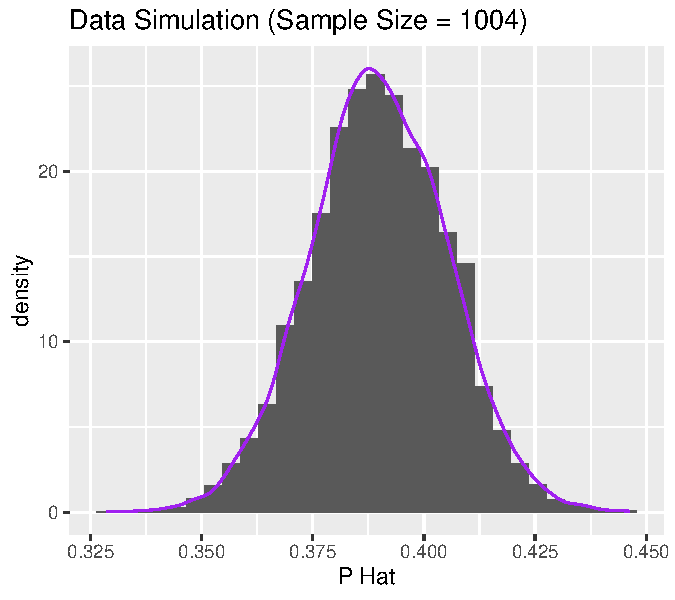
\includegraphics[width=0.435\textwidth]{hhhh.pdf}
\indent 
This histogram is unimodal and is centered around p-hat=0.39. The margin of error comes out to about 3\%, which is actually slightly less than Gallup's margin of error of 4\&. Since our margin of error came out to be a little less than Gallup's, it is possible that they were slightly conservative when reporting their margin of error for their actual sample size.
\newline
\indent 
Now, we can take a look at the histogram showing the sample size of 2008, twice the original size.
\begin{center}
  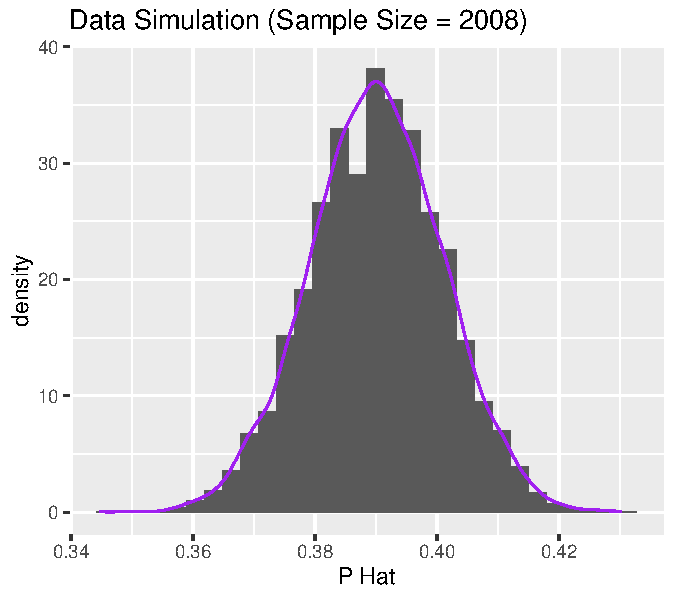
\includegraphics[width=0.435\textwidth]{2008sample.pdf}
\end{center}
\indent 
This histogram looks extremely similiar to the one we just saw. It is also unimodal, and is also centered around p-hat=0.39. For this sample size, the margin of error comes out to just around 2\%, which is what Gallup predicted it would be if they were able to have double the sample size.
\newline
\indent
Unsurprisingly, the resampling histogram seen below looks extremely similiar to the previous two graphs.
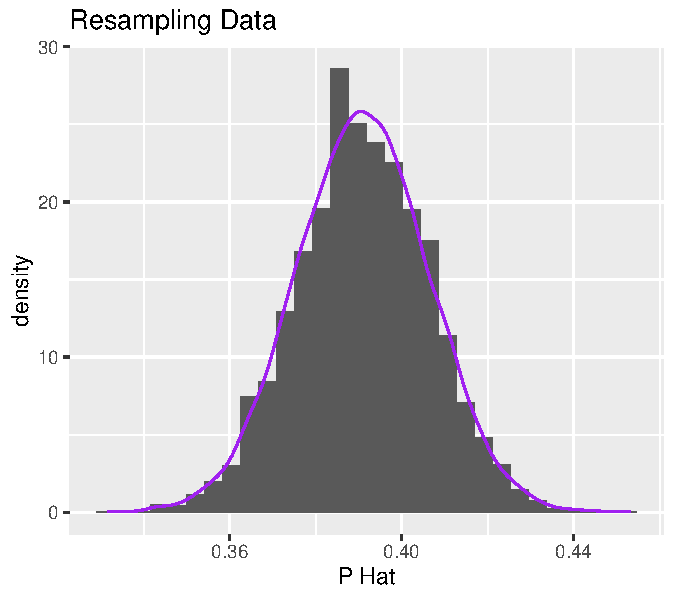
\includegraphics[width=0.435\textwidth]{resampling.pdf}
\indent 
Just like the previous histograms, this one is also unimodal and centered around p-hat=0.39. Similarily to our first simulations graph, the margin of error found by resampling is just about 3\%, which as we saw is slightly lower than Gallup's reported 4\%.
\newline
\indent
Finally, we have the two raster plots which have been combined using \texttt{patchwork} \citep{patchwork}, and placed in the Appendix so that the nuanced differences between the plots can be more easily recognized. Graphically, these two plots appear to be nearly identical, which is because they are in fact nearly identical. For each plot, the margin of error changes in exactly the same was as the sample size and population proportion's each increase. Together, these plots show how running a simulation enough times with a large enough sample size provides us with nearly identical results to the true values found through mathematical calculations. The only difference in the plots is the pixelation which can be seen around the base of the simulation graph. The pixelation is a visual artifact of limited data in the simulation. The math-based plot, however, is built from our theoretical model so it is completely smooth.


\section{Discussion}
This lab explored margin of error in polling data using simulations, resampling, and mathematical calculations. Our findings largely confirmed Gallup's guideline that doubling the sample size from 1000 to 2000 reduces the margin of error from 4\% to 2\%, though our simulation with a sample size of 1004 showed a slightly lower margin of error when compared to Gallup's. Furthermore, our nearly identical side by side raster plots show that when a simulation is run enough times with a large enough sample size, the margin of error it produces is virtually just as accurate as mathematically calculating the true margin of error. These findings back up and reinforce our understanding of the central limit theorem, which tells us that as sample sizes increase, the sampling distribution of the sample proportion becomes approximately normal, allowing both simulation and theoretical methods to converge on the same result.




%%%%%%%%%%%%%%%%%%%%%%%%%%%%%%%%%%%%%%%%%%%%%%%%%%%%%%%%%%%%%%%%%%%%%%%%%%%%%%%%
% Bibliography
%%%%%%%%%%%%%%%%%%%%%%%%%%%%%%%%%%%%%%%%%%%%%%%%%%%%%%%%%%%%%%%%%%%%%%%%%%%%%%%%
\vspace{2em}


\nocite{patchwork}
\nocite{tidyverse}

\begin{tiny}
\bibliography{bib}
\end{tiny}
\end{multicols}

%%%%%%%%%%%%%%%%%%%%%%%%%%%%%%%%%%%%%%%%%%%%%%%%%%%%%%%%%%%%%%%%%%%%%%%%%%%%%%%%
% Appendix
%%%%%%%%%%%%%%%%%%%%%%%%%%%%%%%%%%%%%%%%%%%%%%%%%%%%%%%%%%%%%%%%%%%%%%%%%%%%%%%%
\section{Appendix}
\vspace{-1em} % tighten vertical space
\centering
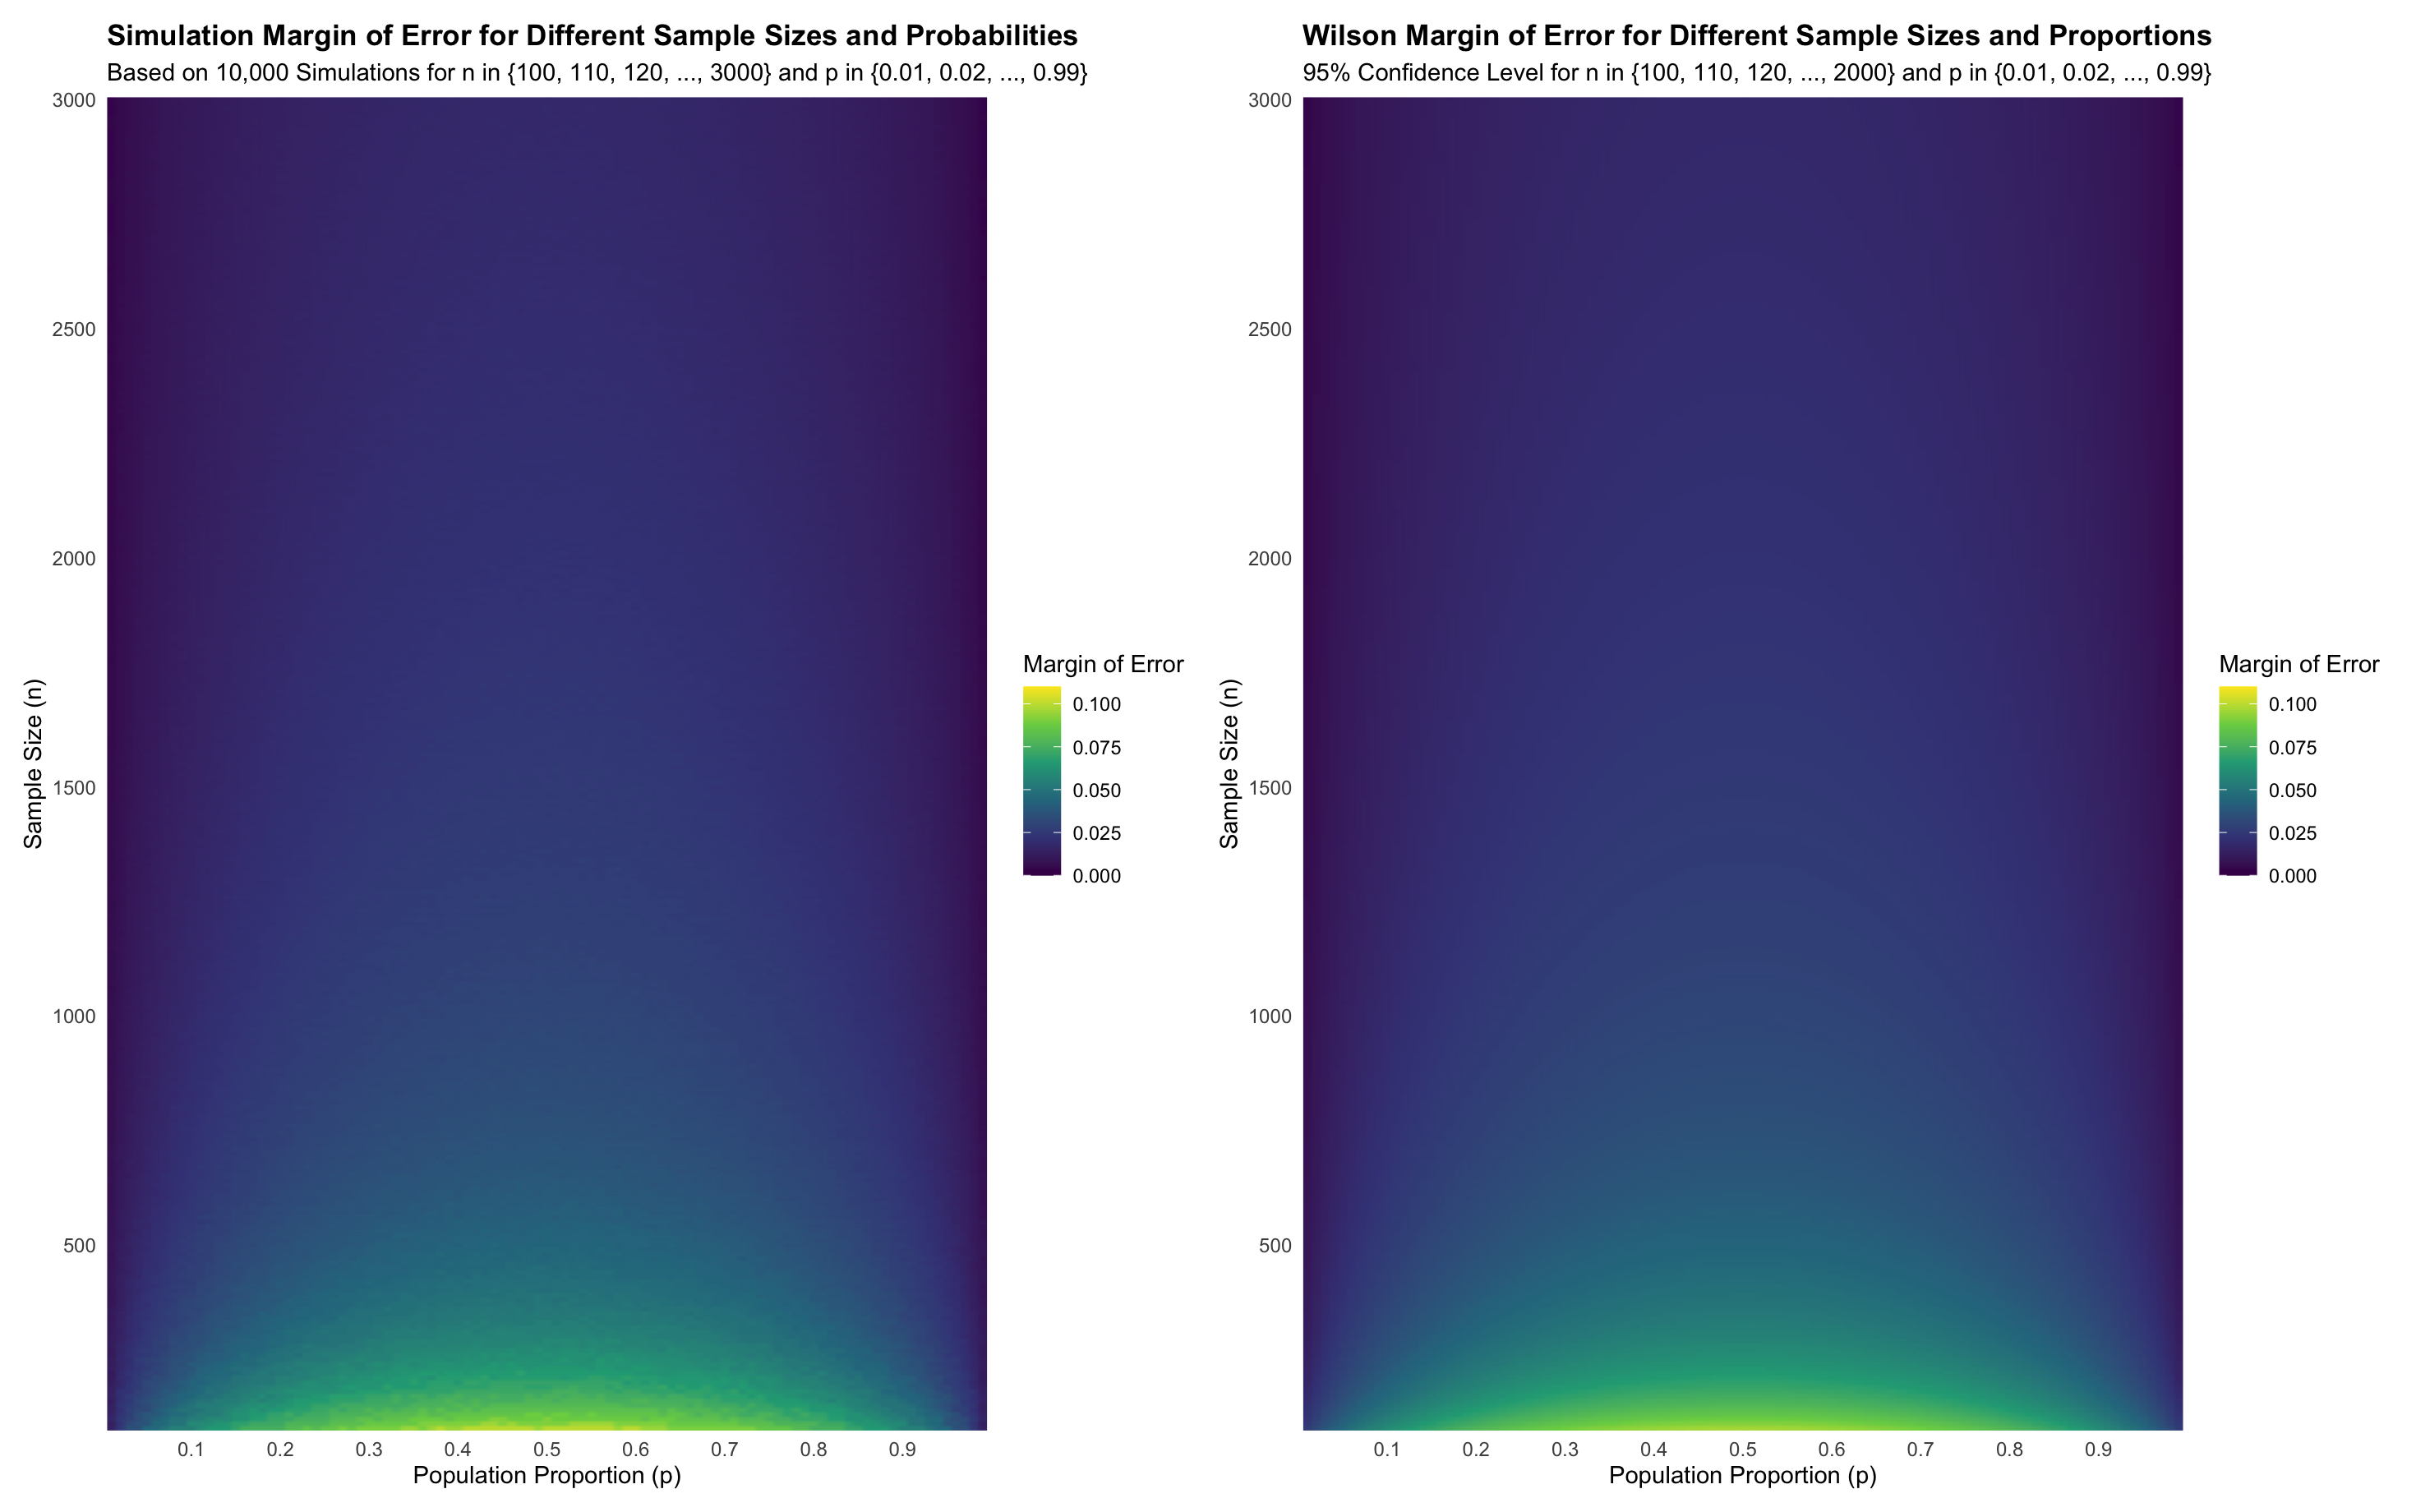
\includegraphics[width=1\textwidth]{Combined.png}
\vspace{-0.5em}
\captionof{figure}{Side by Side Raster Plots Comparing Margin of Error Estimates: Simulation vs. Wilson Formula}


\end{document}
